\Cref{sec:fitting_mbc,sec:background_subtraction} introduced the fitting procedure and \BB background subtraction.
Together with the optimal selections from \Cref{sec:final_optimisation}, this fully defines the analysis strategy from the Belle~II simulated data sets to the \BtoXsgamma spectrum.
However, the defined fit has to be validated in simulation to give an unbiased estimation of \BtoXsgamma events, with a good resolution and signal efficiency.
The studies in this Section prove such results.

\subsection{Validation of \texorpdfstring{\Mbc}{Mbc} fit on reduced samble size}\label{sec:mbc_fit_validation_misreconstructed}

The results in \Cref{fig:mc_fit_yield_comparisons} are obtained by a fit of 1.6~\invab of \MC, which is about an order of magnitude larger than is expected in the case of this analysis.
Therefore, the generic \MC data set is pseudorandomly split into 10 smaller subsets, corresponding to 160~\invfb, and each of them is fitted independently.
The choice of 160~\invfb, rather than 189~\invfb which is the sample size of the Belle~II data used in the analysis, 
is due to anticipated data-simulation differences (see discussion of data-simulation differences in \Cref{sec:corrections}, particularly \FEI calibration in \Cref{sec:fei_calibration}).
Indeed, a 190~\invfb data set corresponds to approximately 160~\invfb in simulation due to differences in tag-\B reconstruction efficiency.

The resulting 10 fits and the estimated $\mathcal{N}_{CB}$ corresponding to each \EB bin are shown in \Cref{fig:extracted_validation_mc}.
The expected number of events in each bin is always equal to one-tenth of that in the generic \MC data set.
It can be observed that all data points, and their average, are statistically compatible with the expectation.
These results indicate that despite using a 10 times larger data set to define the \PDF{s}, this \Mbc fit model produces reliable and stable results.
Further tests, particularly a test ensuring that the fit is unbiased, are performed in \Cref{sec:MC_validation}.

\begin{figure}[htbp!]
    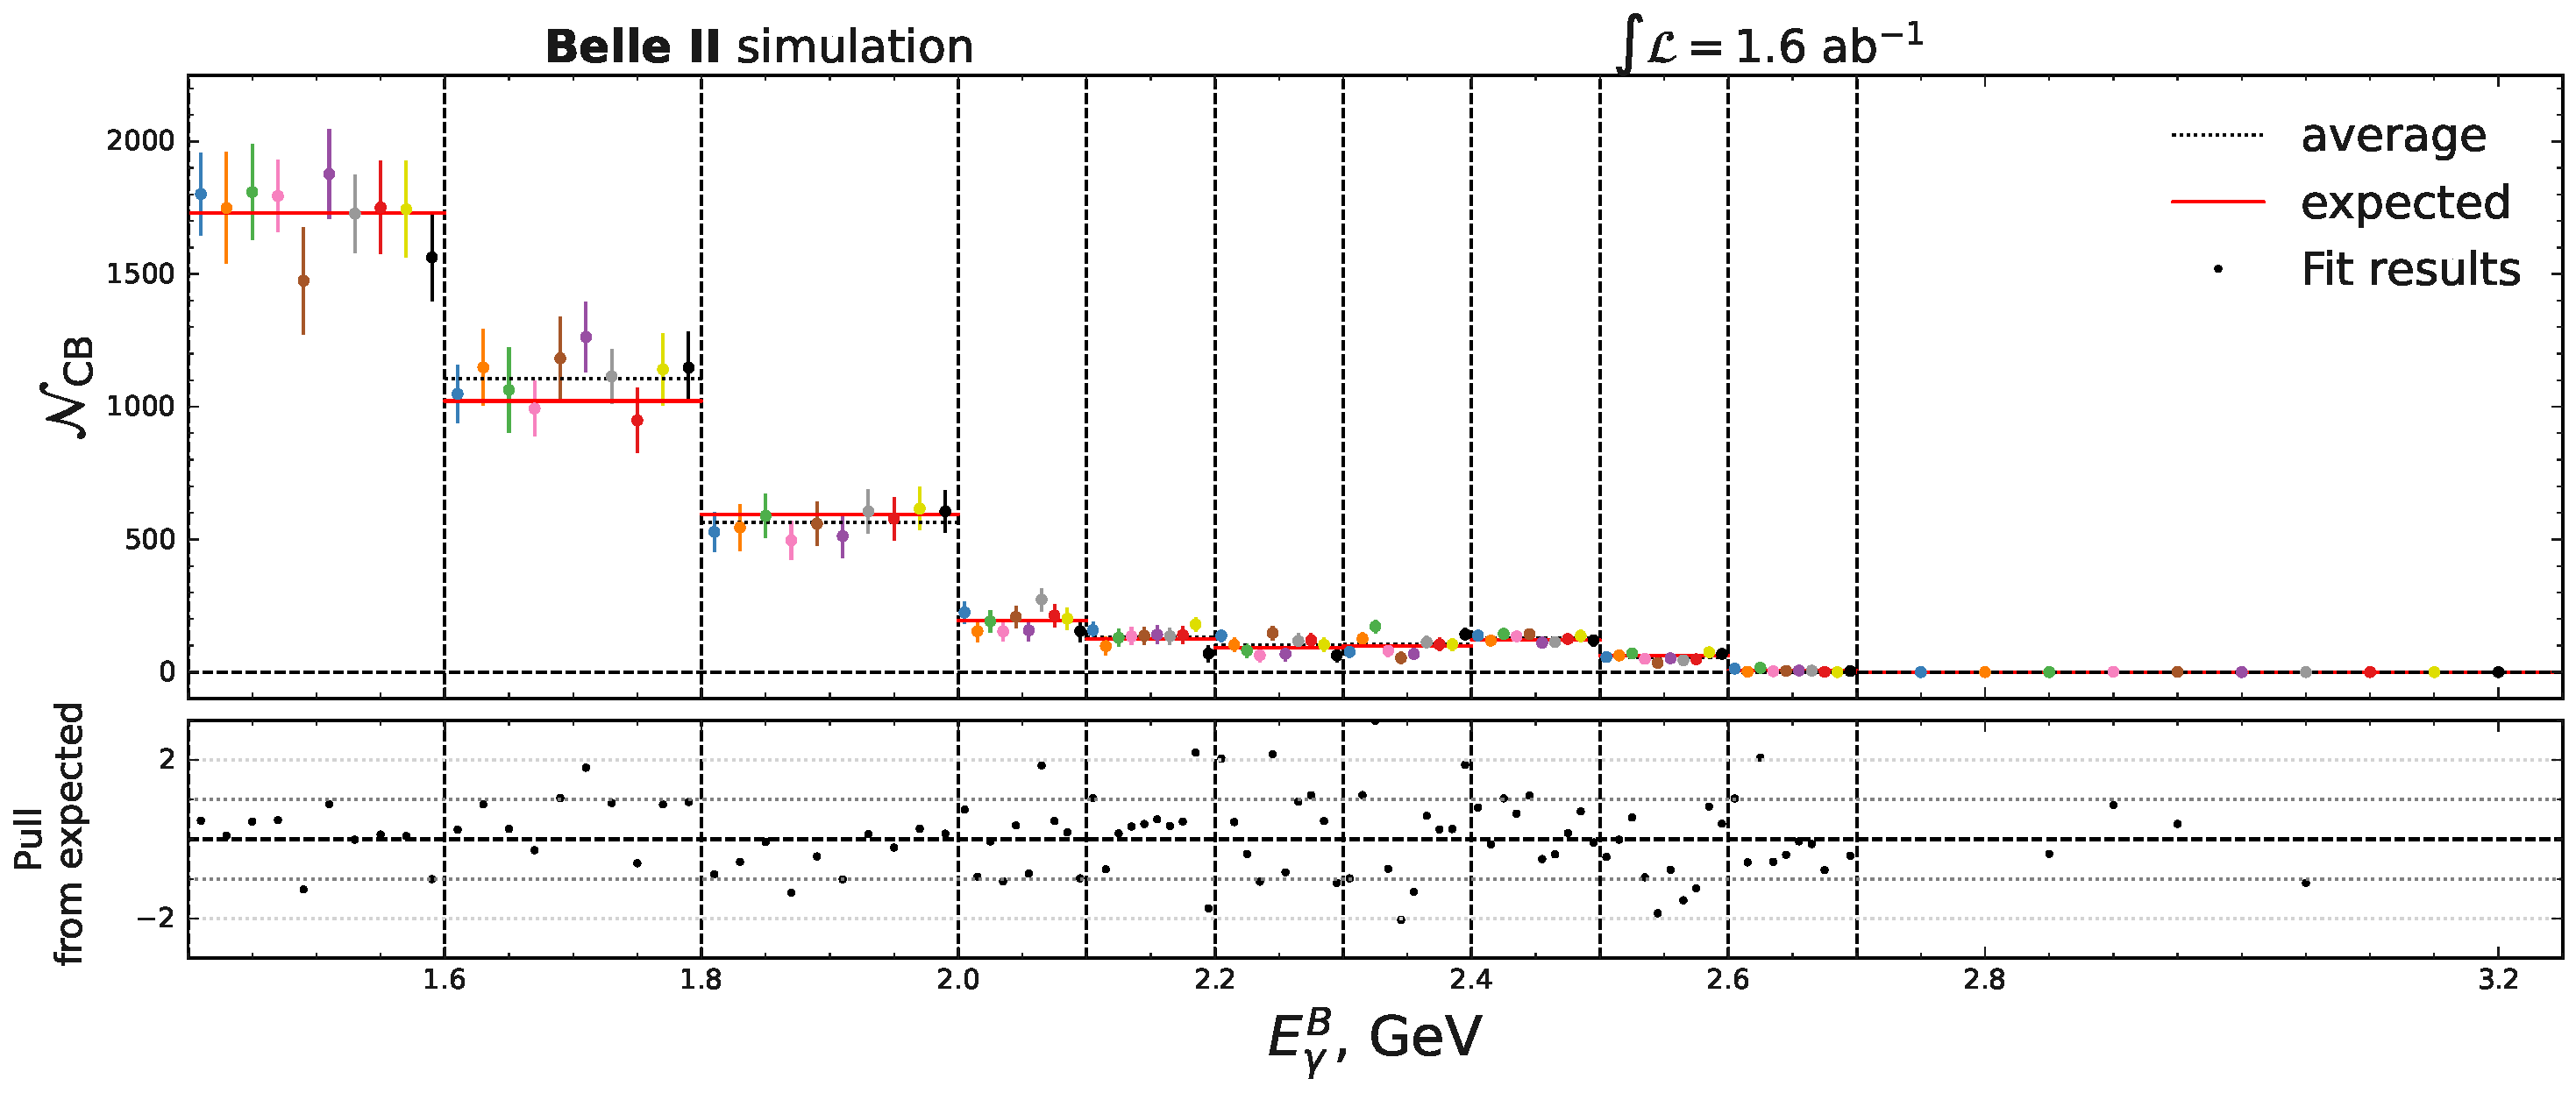
\includegraphics[width=0.9\textwidth]{figures/mc_validation/extracted_signal_generic_mc.pdf}
    \caption{\label{fig:extracted_validation_mc}The estimated $\mathcal{N}_{CB}$ values from fits on one-tenth of generic \MC, corresponding to 160~\invfb of simulation.
    The dashed lines represent different \EB bins, each bin showing one data point corresponding to a simultaneous fit of all \EB bins.
    The dotted lines show the average of all 10 points in each bin, whereas the full lines show the number of good tag-\B events in the original 1.6~\invab data set, scaled down 10 times (`expected').
    The subpanels show the pull of each data point from the expected number of events.
    These results show that the fit extracts a valid result on a data set that is an order of magnitude smaller.
    }
\end{figure}

\subsection{Validation of subtraction of remaining-\texorpdfstring{\BB}{BB} background}\label{sec:background_subtraction_validation_mc}

The strategy to extract the \BtoXsgamma photon energy spectrum and suppress the remaining \BB background was laid out in \Cref{sec:background_subtraction}.
In particular, the full generic \MC data set is modified, such that \BtoXsgamma events are absent from it.
Then, the \Mbc fit discussed in \Cref{sec:fitting_setup} is performed.
To test that this procedure is viable, the subtraction is performed for the results shown in \Cref{fig:extracted_validation_mc}.
Although the 10 fits are performed on 160~\invfb data sets, the background subtraction is done with a 1.6~\invab data set.
Therefore, the statistical uncertainty from the fit on the smaller data set is dominating.
The subtracted result is shown in \Cref{fig:subtracted_validation_mc}.

\begin{figure}[htbp!]
    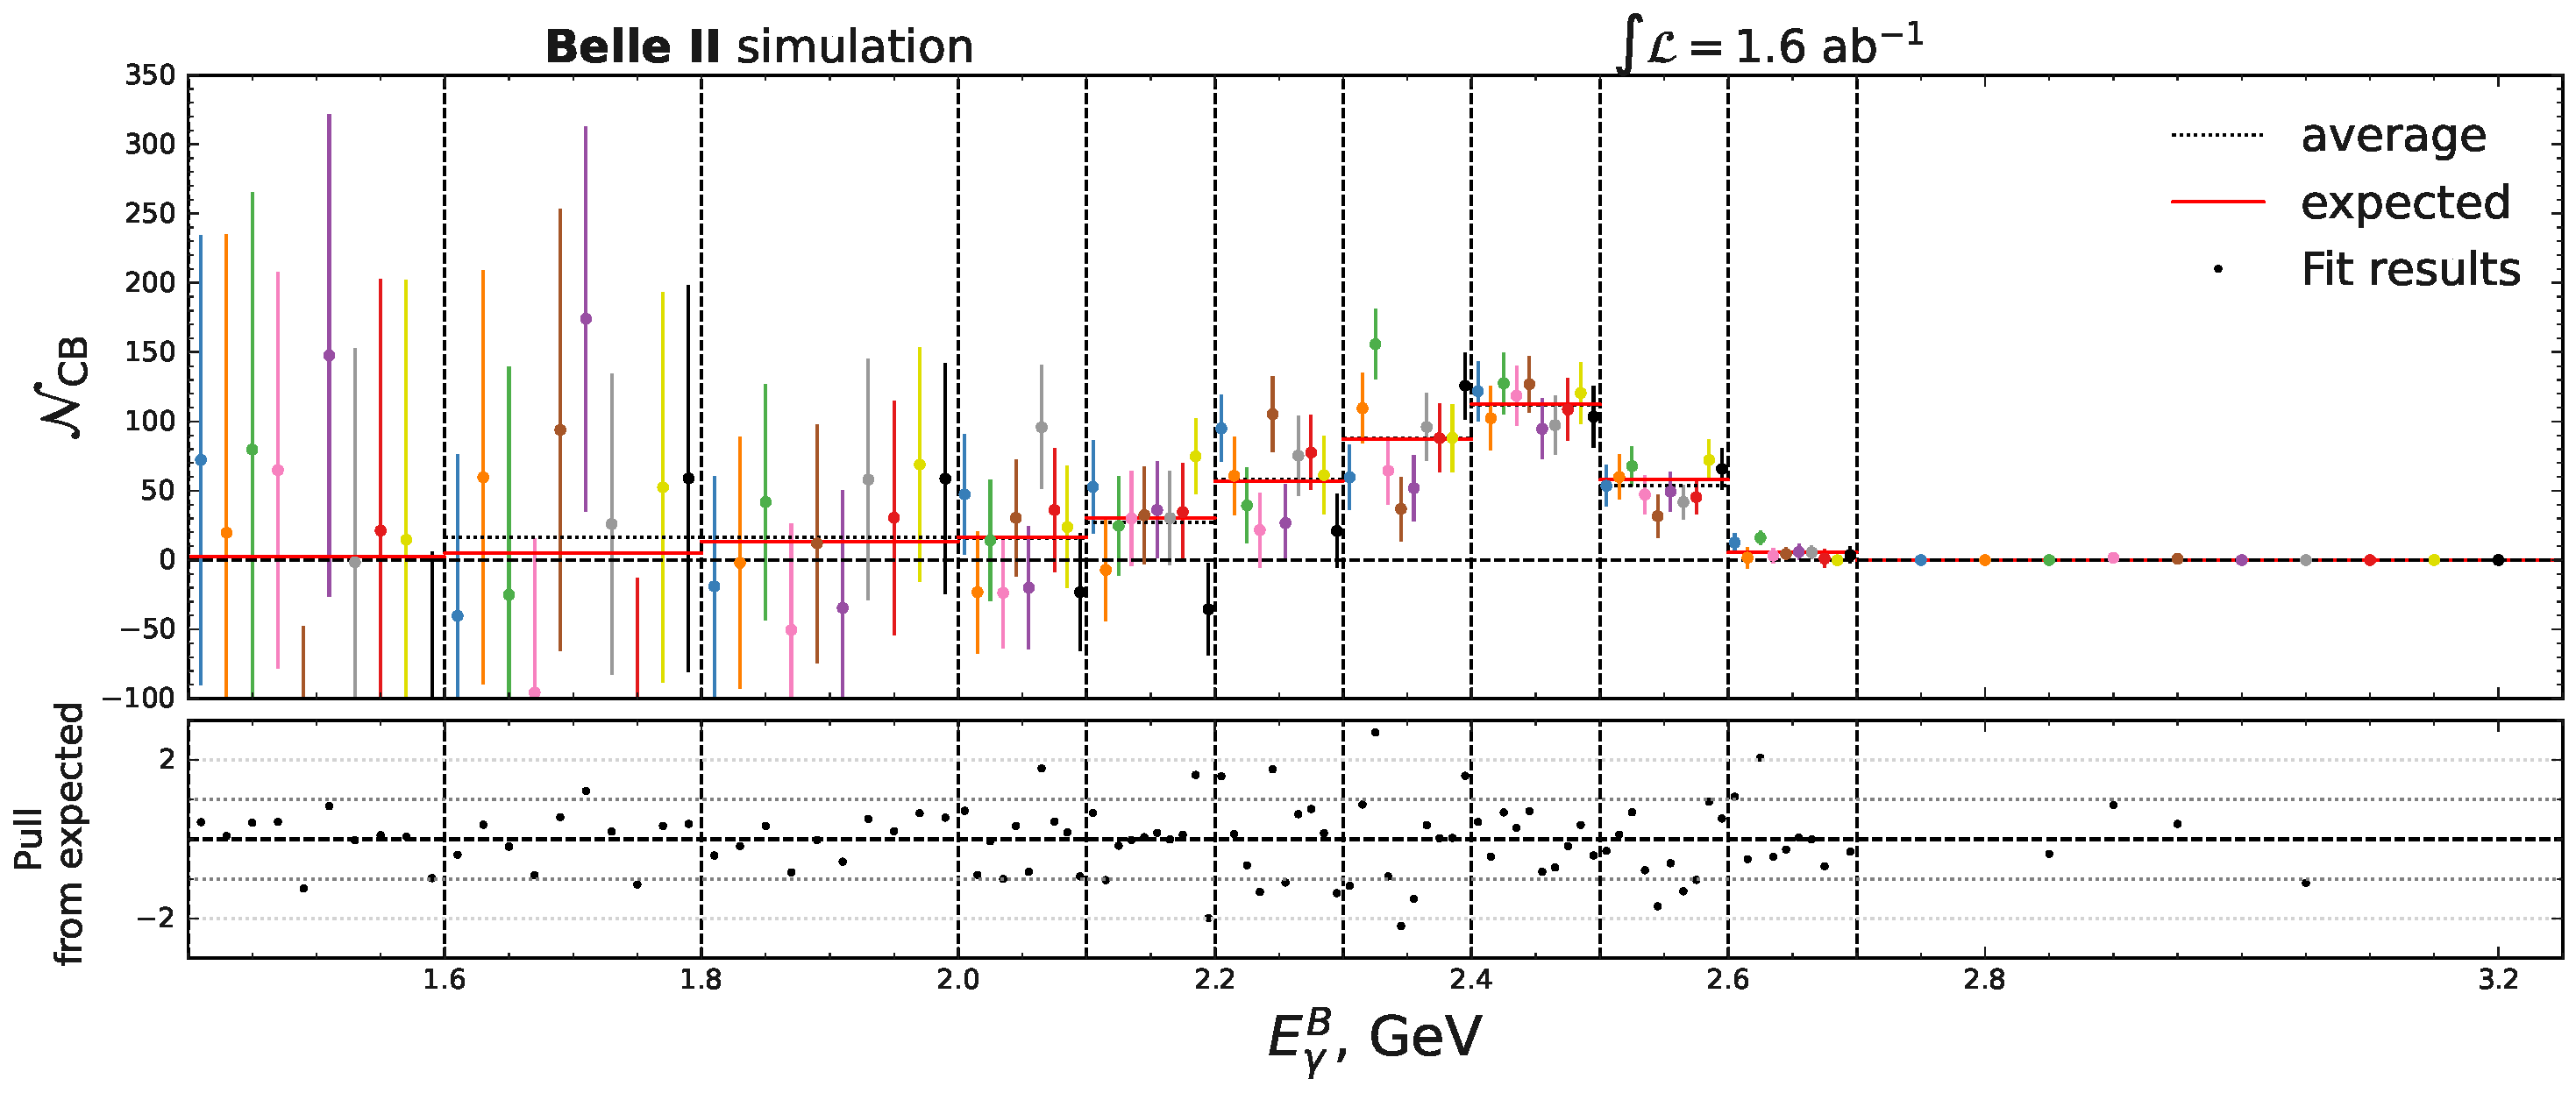
\includegraphics[width=0.9\textwidth]{figures/mc_validation/subtracted_signal_generic_mc.pdf}
    \caption{\label{fig:subtracted_validation_mc}
    The estimated $\mathcal{N}_{CB}$ with subtracted background, based on the \Cref{eq:background_subtraction}.
    The values before \BB-background subtraction are shown in a corresponding \Cref{fig:extracted_validation_mc}.
    The peak is the presence of \BtoXsgamma events in \MC, and can be seen to agree well with the generic \MC expectations.
    To ensure that minimal statistical background subtraction uncertainty is introduced, the full 1.6~\invab data set is chosen to subtract the background.
    The uncertainties of each data point are those of the \Mbc fit on the background data set and on the tested subset, added in quadrature.
    }
\end{figure}

The 1.6~\invab data set and the 160~\invfb subsets are largely correlated, therefore the result has a smaller spread than one might expect from a unit Gaussian, based on the statistical uncertainty provided by the fit.
However, the purpose of this test is to showcase that the setup extracts values that are statistically compatible with the scaled-down original data set.
The results showcased in \Cref{fig:extracted_validation_mc,fig:subtracted_validation_mc} clearly show that the central values of the \EB spectrum extracted follow the number of \BtoXsgamma events in the data set.
In this Section so far, no particular modelling of \BtoXsgamma spectrum has been assumed.
On the other hand, following the setup that is taken to remove \BB backgrounds after the \Mbc fit, the analysis is heavily dependent on the background model.
For this reason, special emphasis will be put on testing the \textit{background} description validation in \Cref{sec:corrections,sec:validation}.

\subsection{Closure test of the \texorpdfstring{\Mbc}{Mbc} fit}\label{sec:closure_test}

If the uncertainties estimated by a fit are correct, then fitting pseudodata sets generated from \PDF{s} fitted on test data must yield statistically compatible results.
This verifies two important aspects of the fit:
\begin{itemize}
    \item the estimated fit parameter central values are reproduced when fitting a statistically equivalent data set;
    \item the estimated fit parameter uncertainties appropriately describe the statistical fluctuations of the central values.
\end{itemize}

More concisely, the pull distribution of an unbiased fit, in this case, calculated as:
\begin{equation}\label{eq:toy_pull}
    \mathrm{pull} = \frac{\mathcal{N}_{\mathrm{CB}}\cdot \mathrm{scale} - \mathcal{N}_{\mathrm{CB}}^{\mathrm{pseudo}}}{\mathrm{fit~error}},
\end{equation}
must be described by a unit Gaussian (assuming the central limit theorem is applicable for the pseudodata sample size).
In the case of this analysis, $\mathcal{N}_{\mathrm{CB}}$ is the estimated number of good tag-\B mesons in the generic \MC sample.
On the other hand, $\mathcal{N}^{\mathrm{pseudo}}_{\mathrm{CB}}$ are the normalisations estimated in a a randomly sampled data set that follows the \PDF{s} fitted on the generic \MC data set.
The $\mathrm{fit~error}$ is the corresponding uncertainty, in this analysis estimated by the \texttt{HESSE} method.
The $\mathrm{scale}$ is used to equate the sample size between the sampled and total simulated data set.
Tests of this type are known as \textit{closure tests} and allow verifying that the central values reproduced by the fit fluctuate as indicated by the \PDF uncertainties.

The closure test in this analysis is done on pseudodata sets of equivalent size as the Belle~II collected data.
First, 1000 pseudodata sets equivalent to $\mathrm{160~\invfb}$ are sampled from the \PDF that was fitted in \Cref{fig:primary_full_fits}.
Since in all of the cases $\mathcal{N}_{\mathrm{CB}}$ and $\mathrm{fit~error}$ are known, the \Mbc fit is used on the pseudodata set, and a $\mathrm{pull}$ is calculated based on \Cref{eq:toy_pull}.
The pull distributions for every \EB bin are shown in \Cref{fig:pull_distributions}.

\begin{figure}[htbp!]
    \centering
    \subcaptionbox{\label{fig:pulls_1p4to1p6}}{
        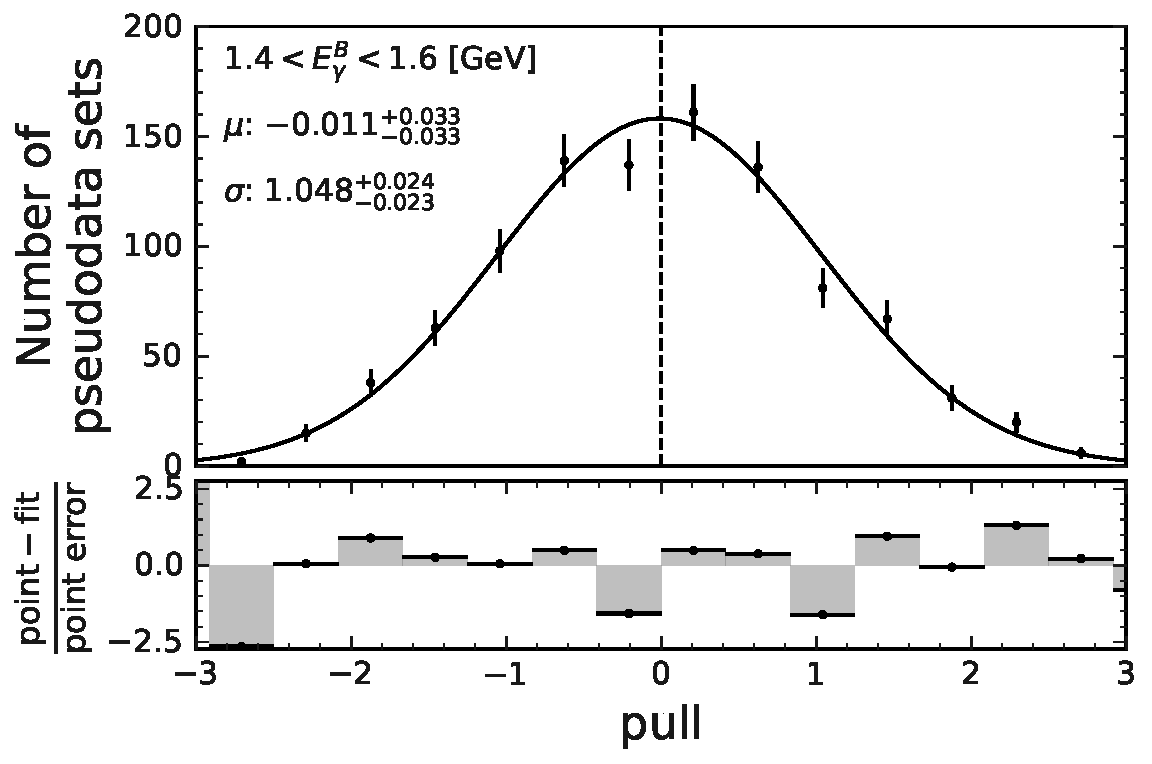
\includegraphics[width=0.31\textwidth]{figures/mc_validation/toy_study/fits_of_pulls_1p4to1p6.pdf}
    }
    \subcaptionbox{\label{fig:pulls_1p6to1p8}}{
        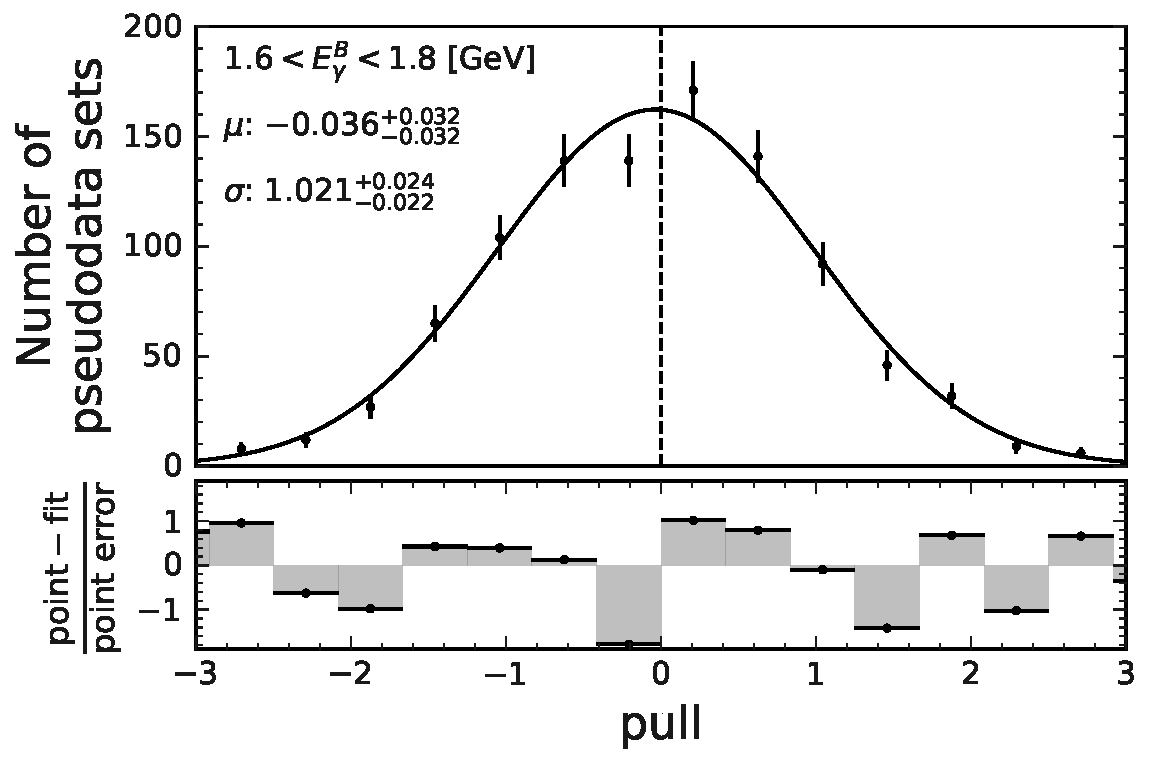
\includegraphics[width=0.31\textwidth]{figures/mc_validation/toy_study/fits_of_pulls_1p6to1p8.pdf}
    }
    \subcaptionbox{\label{fig:pulls_1p8to2p0}}{
        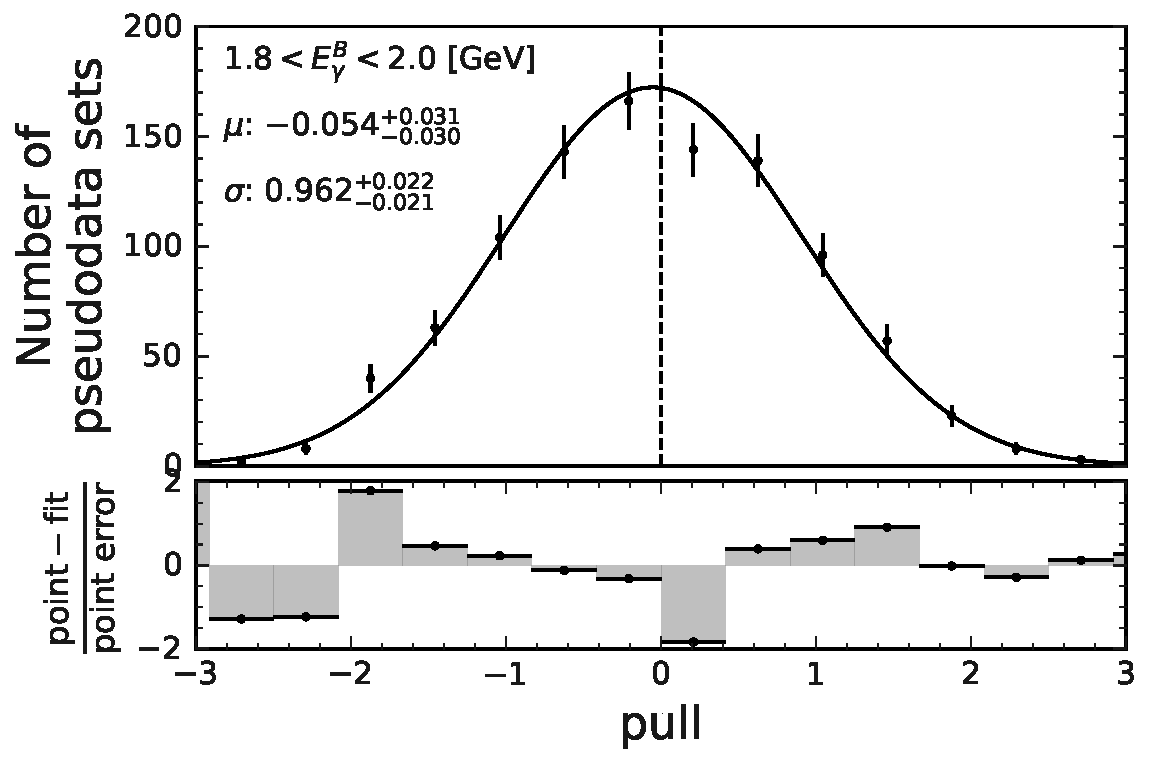
\includegraphics[width=0.31\textwidth]{figures/mc_validation/toy_study/fits_of_pulls_1p8to2p0.pdf}
    }
    \subcaptionbox{\label{fig:pulls_2p0to2p1}}{
        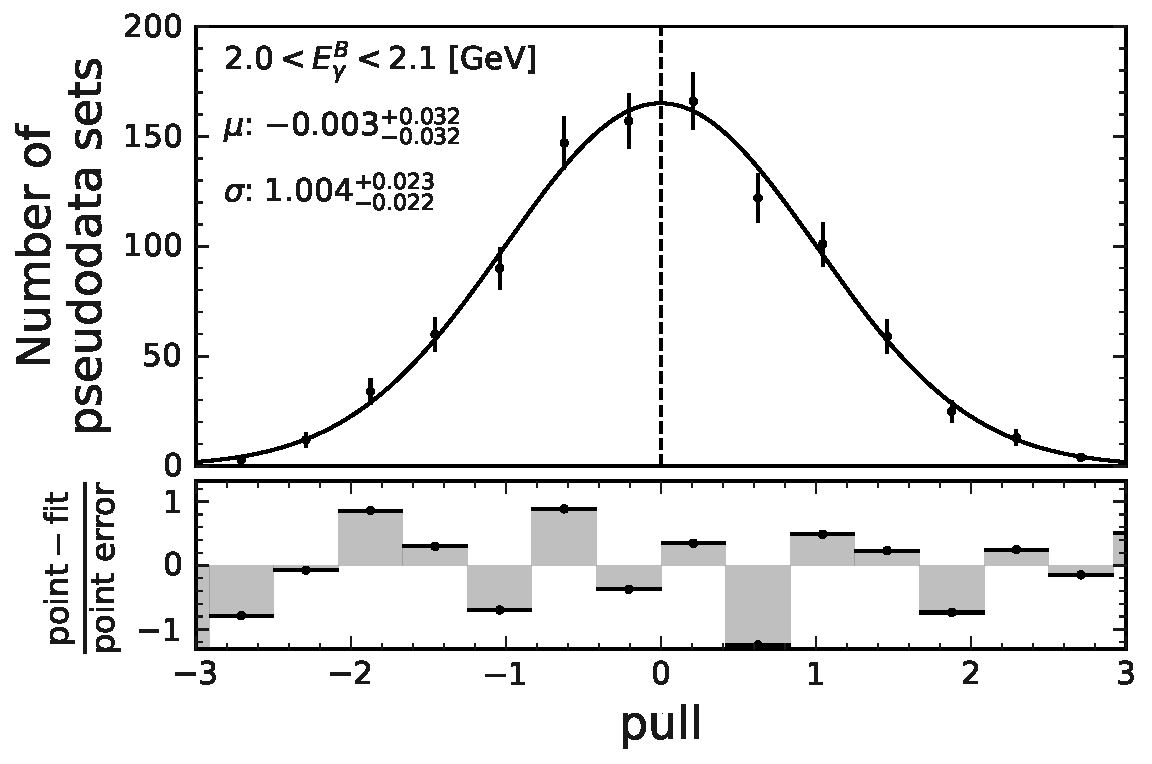
\includegraphics[width=0.31\textwidth]{figures/mc_validation/toy_study/fits_of_pulls_2p0to2p1.pdf}
    }
    \subcaptionbox{\label{fig:pulls_2p1to2p2}}{
        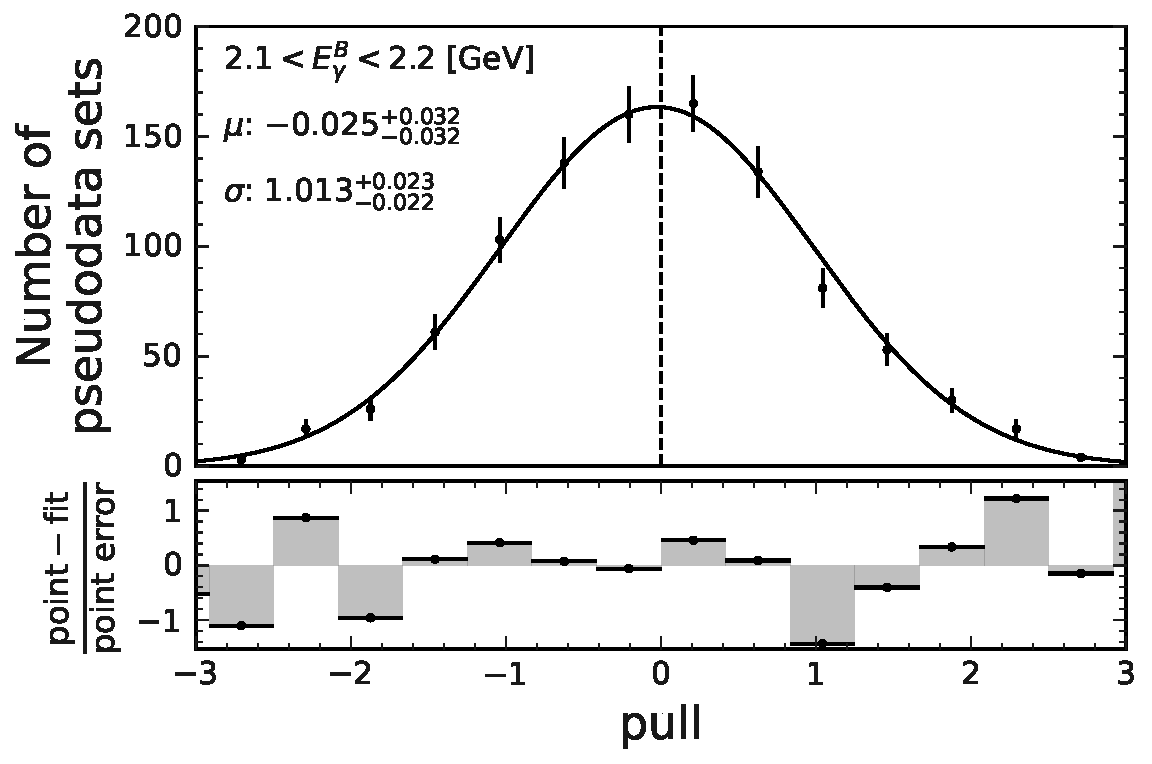
\includegraphics[width=0.31\textwidth]{figures/mc_validation/toy_study/fits_of_pulls_2p1to2p2.pdf}
    }
    \subcaptionbox{\label{fig:pulls_2p2to2p3}}{
        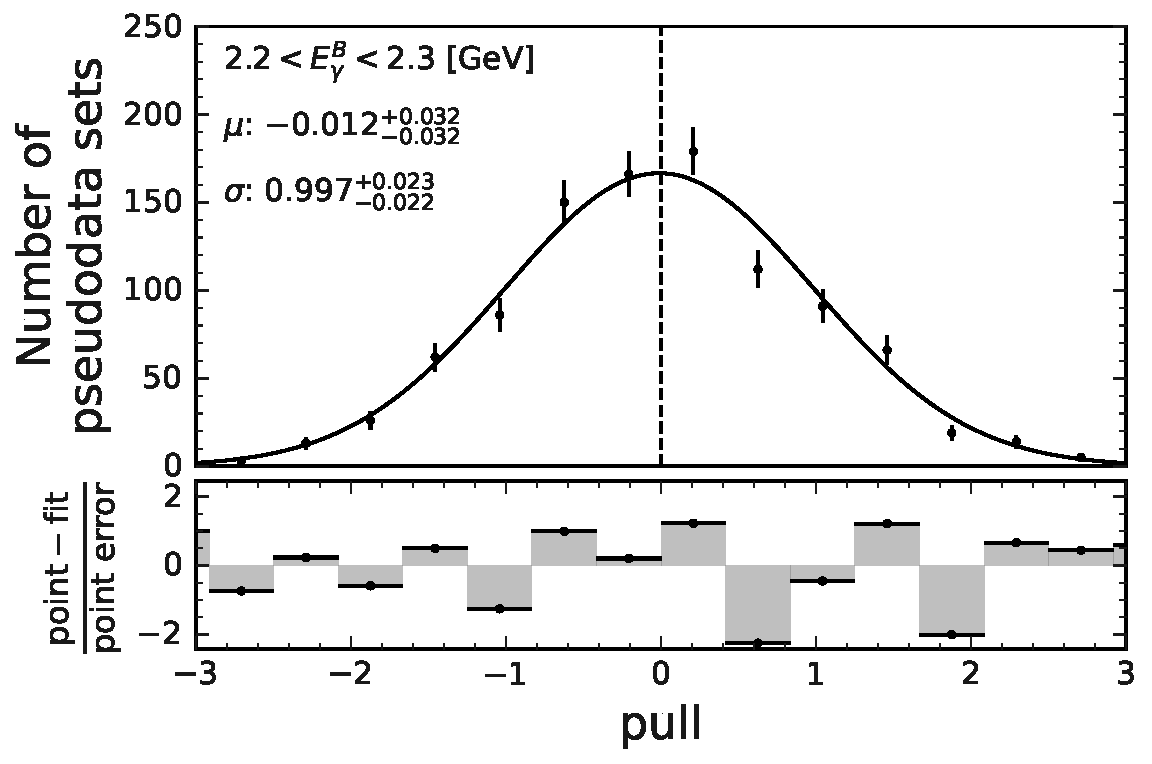
\includegraphics[width=0.31\textwidth]{figures/mc_validation/toy_study/fits_of_pulls_2p2to2p3.pdf}
    }
    \subcaptionbox{\label{fig:pulls_2p3to2p4}}{
        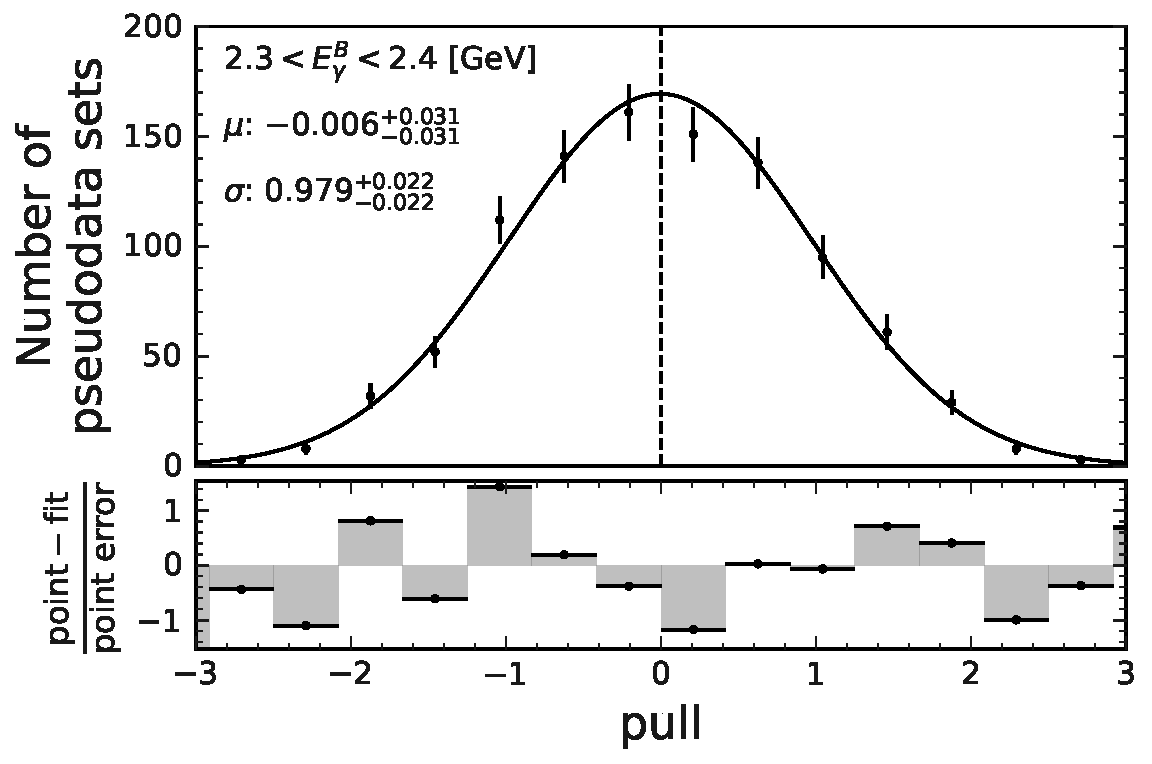
\includegraphics[width=0.31\textwidth]{figures/mc_validation/toy_study/fits_of_pulls_2p3to2p4.pdf}
    }
    \subcaptionbox{\label{fig:pulls_2p4to2p5}}{
        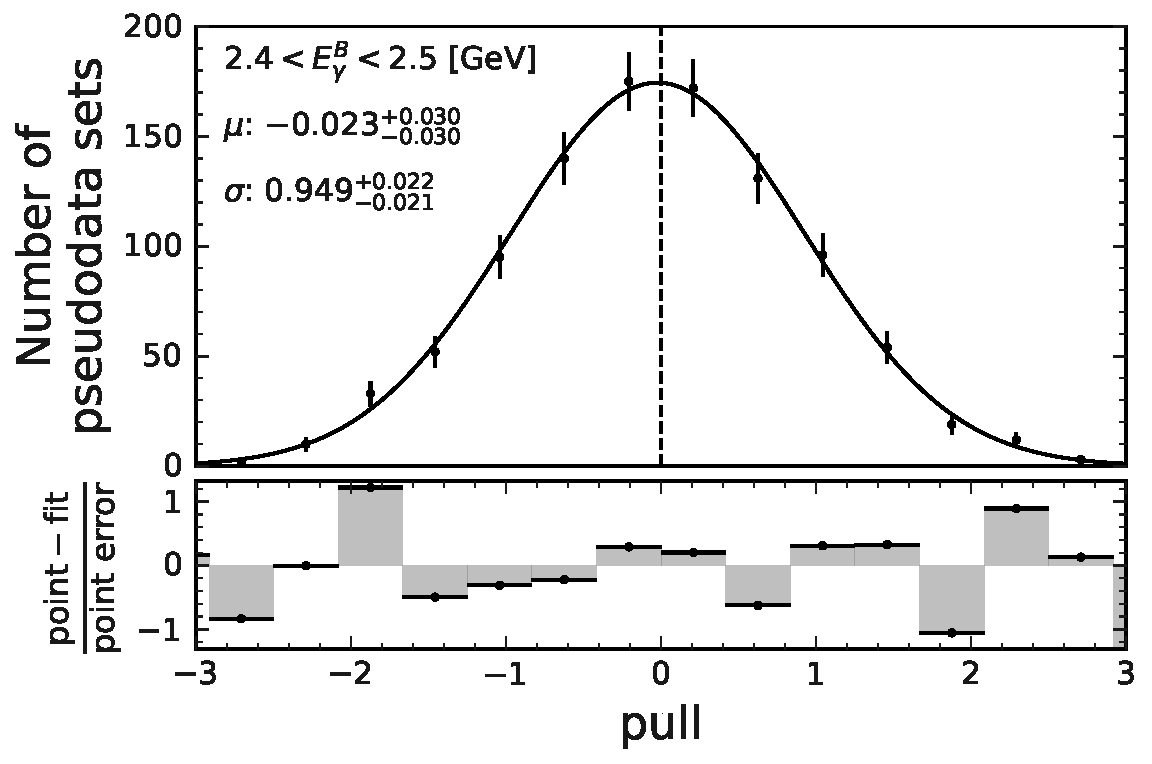
\includegraphics[width=0.31\textwidth]{figures/mc_validation/toy_study/fits_of_pulls_2p4to2p5.pdf}
    }
    \subcaptionbox{\label{fig:pulls_2p5to2p6}}{
        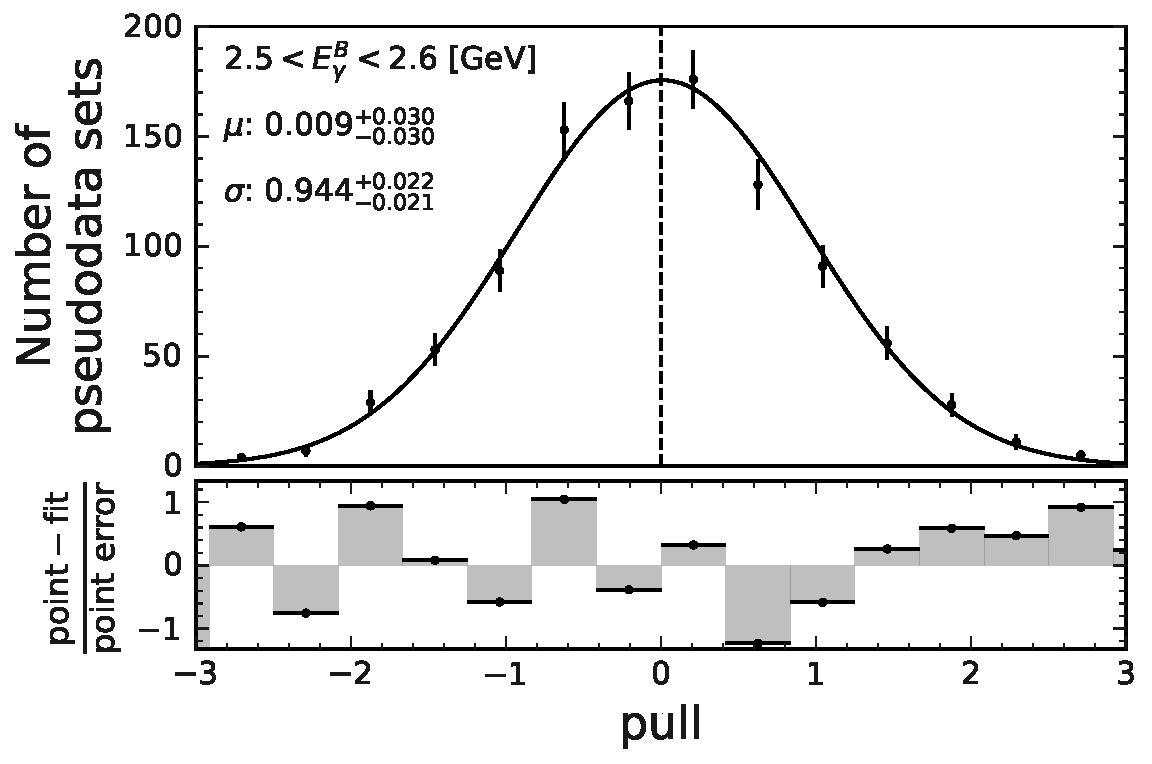
\includegraphics[width=0.31\textwidth]{figures/mc_validation/toy_study/fits_of_pulls_2p5to2p6.pdf}
    }
    \subcaptionbox{\label{fig:pulls_2p6to2p7}}{
        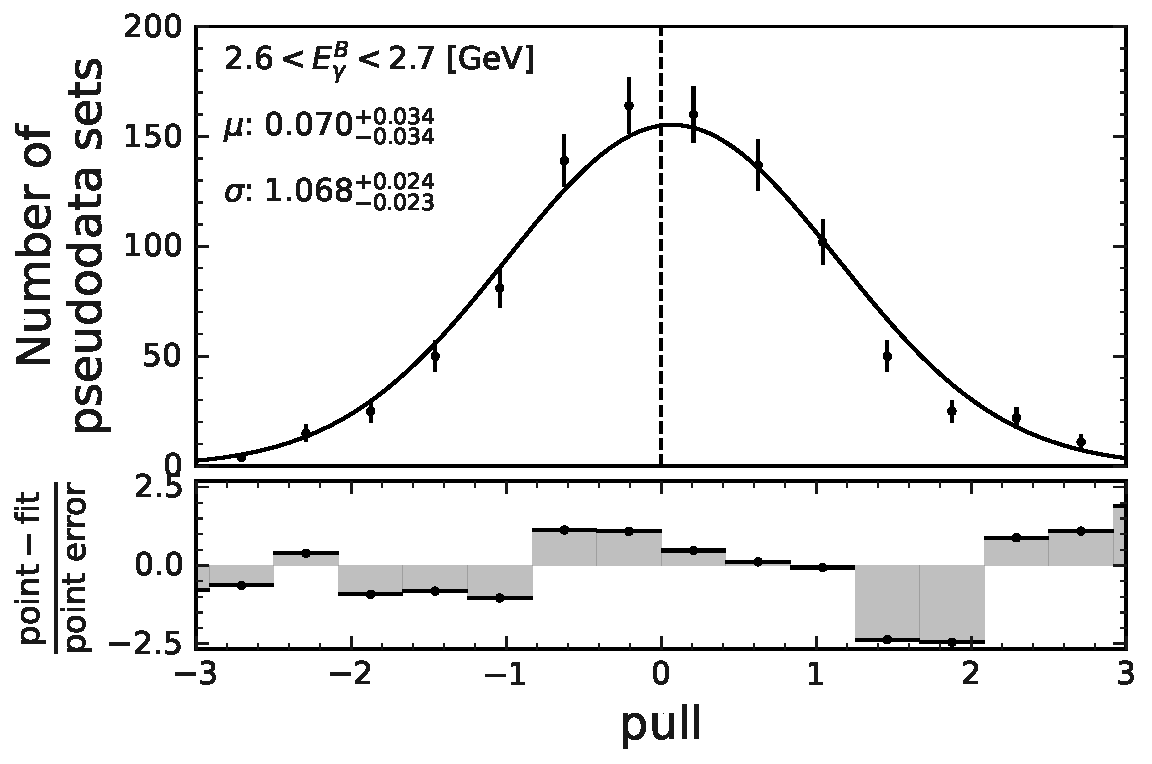
\includegraphics[width=0.31\textwidth]{figures/mc_validation/toy_study/fits_of_pulls_2p6to2p7.pdf}
    }
    \subcaptionbox{\label{fig:pulls_2p7to5p0}}{
        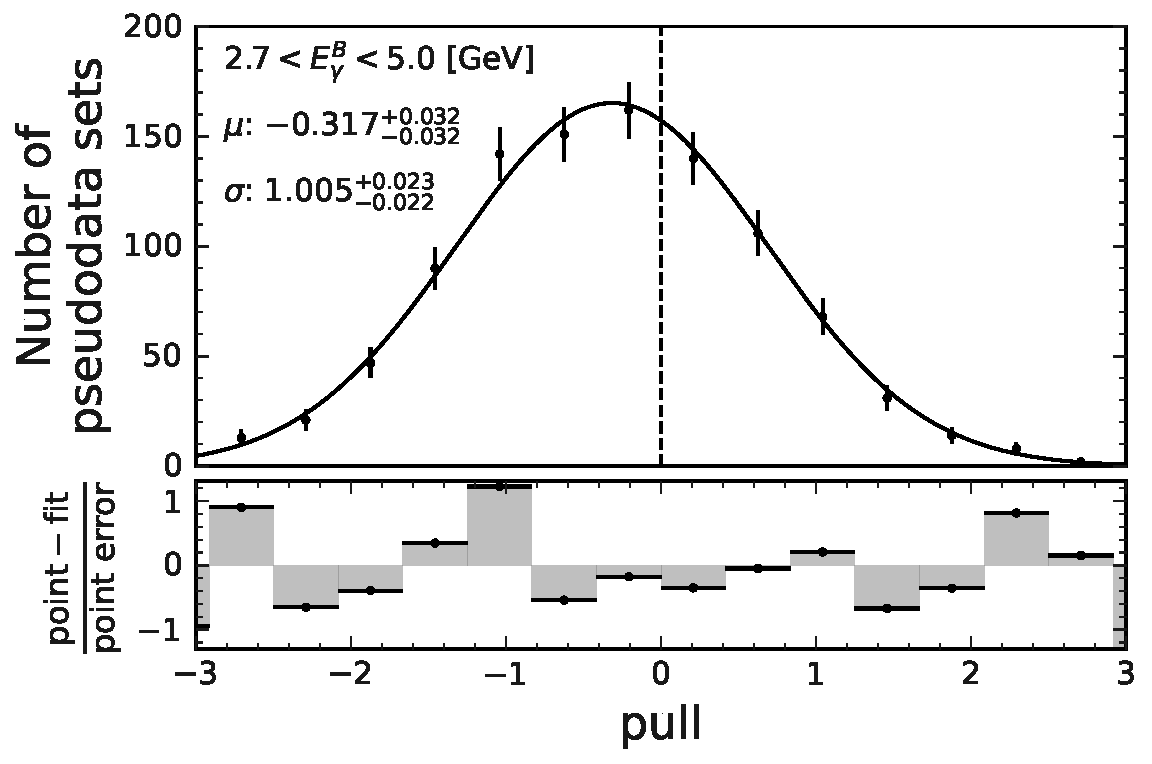
\includegraphics[width=0.31\textwidth]{figures/mc_validation/toy_study/fits_of_pulls_2p7to5p0.pdf}
    }
    \caption{\label{fig:pull_distributions}The pull distributions used in the \Mbc fit closure test, 
    corresponding to results of 1000 pseudodata sets generated based on the \PDF fitted on the total generic \MC data set.
    The definition of the pull for this test is given in \Cref{eq:toy_pull}.
    The data points show the counts of values in the given pull intervals, and the statistical uncertainty.
    The pulls are also fitted with a Gaussian distribution and the mean value, $\mu$, as well as the width, $\sigma$, are extracted.
    The Gaussian fit is shown as a solid line and is an unbinned fit (i.e. not the fit to the shown data points).
    }
\end{figure}

To test the statistical validity of \Mbc fits in each bin, a Gaussian \PDF is fitted on the distributions, with parameters $\mu$ and $\sigma$ being estimated.
The parameters correspond to the mean value and the width of the Gaussian distribution, respectively.
The parameter estimation is performed as an unbinned negative log-likelihood fit.
The corresponding Gaussian fit results and the parameters are also included in \Cref{fig:pull_distributions} and also summarised in \Cref{fig:mean_sigma_pulls}.
\begin{figure}[htbp!]
    \centering
    \subcaptionbox{\label{fig:mean_pulls}}{
        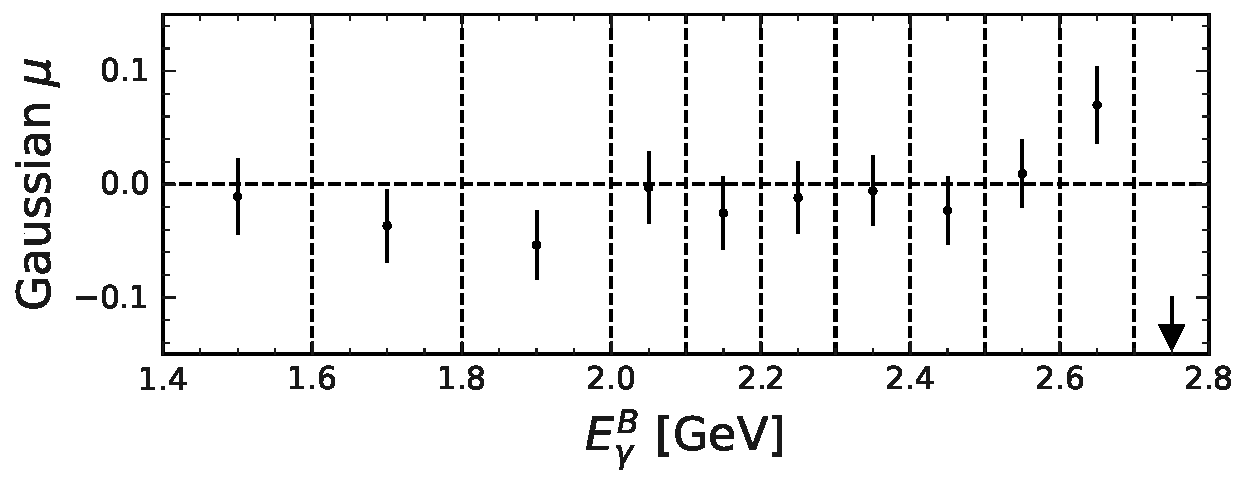
\includegraphics[width=0.45\textwidth]{figures/mc_validation/toy_study/mean_pull_toys.pdf}
    }
    \subcaptionbox{\label{fig:sigma_pulls}}{
        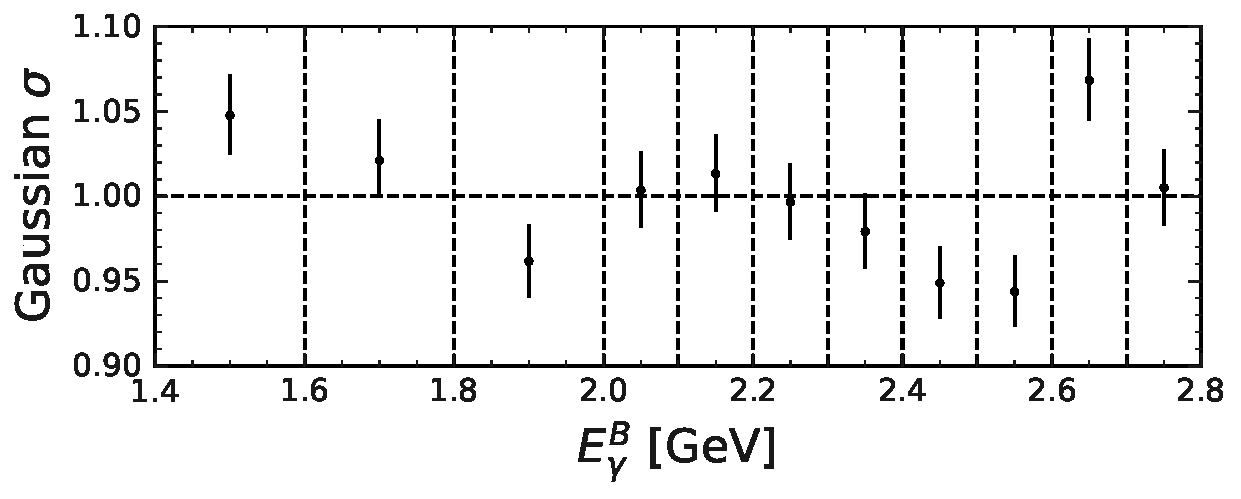
\includegraphics[width=0.45\textwidth]{figures/mc_validation/toy_study/sigma_pull_toys.pdf}
    }
    \caption{\label{fig:mean_sigma_pulls}Summarised means and widths ($\mu$ and $\sigma$, respectively) of the Gaussian fits of
    the pull distributions in each \EB bin.
    The fits for evaluation of $\mu$ and $\sigma$ are shown in \Cref{fig:pull_distributions}.
    The results are compatible with a unit Gaussian except in the case of parameter $\mu$ for \mbox{$\EB>2.7~\gev$}, where statistical effects play a large role.
    }
\end{figure}

In all cases the results are compatible with a unit Gaussian within to 2 standard deviations.
As the pulls distributions are Gaussian-like, the central limit theorem regime is reached.
The only exception is the parameter $\mu$  in $\EB>2.7~\gev$.
Here, the central value of the pulls appears to be biased towards lower values.
This is attributed to statistical effects, as that bin has only a handful of entries (even at 1.6~\invab) and is therefore strongly affected by statistical background fluctuations.
As it is not expected to observe any statistically significant signal events in that region, it is chosen to not define any correction based on the observed bias.

These results allow concluding that the \Mbc fit is an unbiased estimator.
In other words, the central values are unbiased and the uncertainties adequately cover the statistical fluctuations of the results.

\subsection{Linearity test of the \texorpdfstring{\Mbc}{Mbc} fit}\label{sec:linearity_test}

The fit is further validated using the so-called \textit{linearity} test.
Any valid extended fit model ought to provide a behaviour such that the estimated normalisation, $\mathcal{N}$, grows linearly with the increase of the corresponding component in the fitted data set.
To perform such a test in this analysis, up to 25000 \BtoXsgamma signal-\MC events where a good tag-\B meson has been identified are combined with the generic \MC data set.
For a valid fitting setup, $N$ events `injected' in the fitted data set should yield approximately an increase of $N$ in the estimated $\mathcal{N}_{\mathrm{CB}}$.
Such a test of the expected linear behaviour is summarised in \Cref{fig:linearity_test}.

\begin{figure}[htbp!]
    \centering
    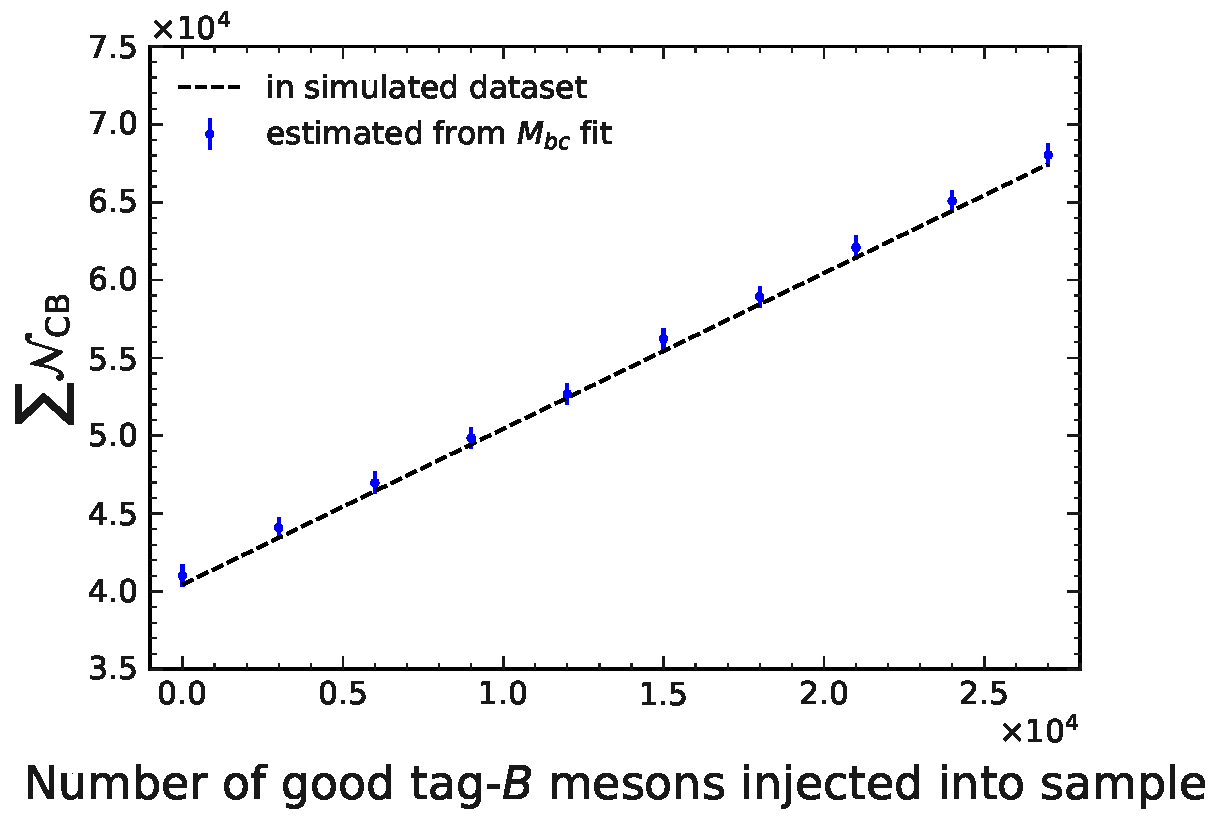
\includegraphics[width=0.45\textwidth]{figures/mc_validation/linearity_check_longer.pdf}
    \caption{\label{fig:linearity_test}The summary of the linearity test for the \Mbc fit of this analysis.
    As the number of events corresponding to the peaking tag-\B mesons increases, the extracted sum of normalisations across all bins, $\Sigma\mathcal{N}_{\mathrm{CB}}$, also increases.
    The increase is compatible with a linear increase with a slope of unity.
    }
\end{figure}

As the number of `injected' good tag-\B events grows, the sum of the normalisations for all \EB bins should increase linearly.
This behaviour is reproduced, as $\sum \mathcal{N}_{\mathrm{CB}}$ grows linearly with the increase of the data set.
It can therefore be concluded that the behaviour of the \Mbc fit is linear.

\subsection{Correlation matrix of the parameters of the \texorpdfstring{\Mbc}{Mbc} fit}\label{sec:correlation_matrix}

Using the pseudodata sets generated in \Cref{sec:closure_test}, relationships between all parameters estimated by the \Mbc fit can be calculated.
In particular, a Pearson-R correlation coefficient for some collection of paired values ${(x_1,y_1),(x_2,y_2,)...,(x_n,y_n)}$:
\begin{equation}\label{eq:pearson_r}
    R_{x,y}=\frac{\sum_{i=1}^n\left(x_i-\bar{x}\right)\left(y_i-\bar{y}\right)}{\sqrt{\sum_{i=1}^n\left(x_i-\bar{x}\right)^2} \sqrt{\sum_{i=1}^n\left(y_i-\bar{y}\right)^2}}.
\end{equation}

For every pair of parameters estimated by the \Mbc fit, the Pearson-R value is evaluated.
This results in a 36-by-36 matrix, corresponding to all parameters estimated by the \Mbc fit in this analysis, and shown in \Cref{fig:correlation_matrix}.
The 37th parameter, $m_0$, is not included, because no significant correlations with that parameter are observed in the fit.
\begin{figure}[htbp!]
    \centering
    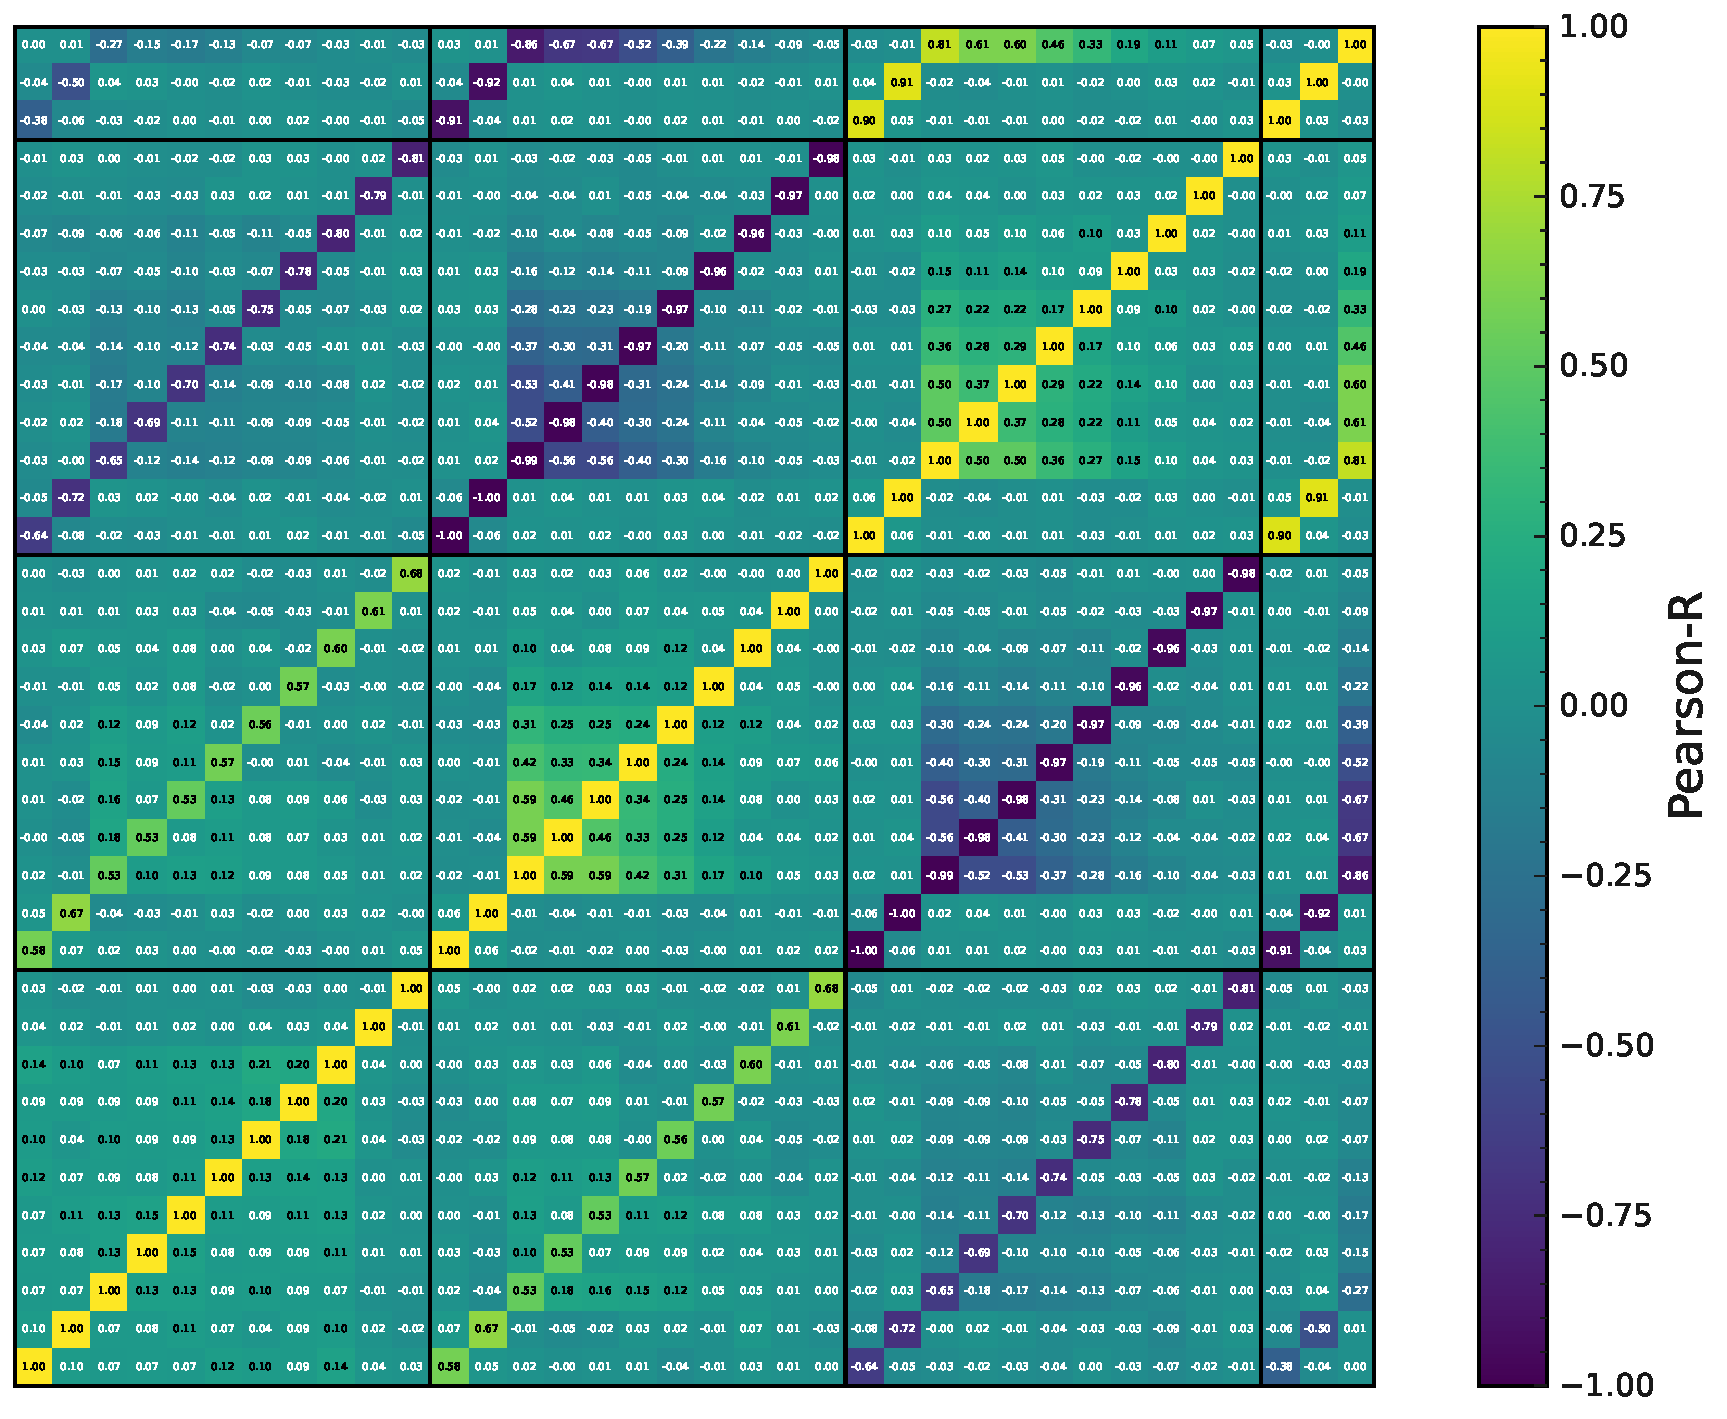
\includegraphics[width=1.1\textwidth]{figures/mc_validation/correlation_matrix.pdf}
    \caption{\label{fig:correlation_matrix}The correlation matrix of the \Mbc fit, generated using a 1000 pseudodata set.
    Every pair of parameters has their correlation evaluated as the Pearson-R coefficient (\Cref{eq:pearson_r}).
    Parameter names correspond to those in \Cref{tab:fitting_init_params} and the numbering $0-10$ correspond to the bin number, starting from $1.4-1.6~\gev$.
    }
\end{figure}

Several important insights into the fit can be understood by observing the correlation matrix:
\begin{itemize}
\item
Firstly, consider the correlation of ${\mathcal{N}_{\mathrm{CB}}}_{i}$ with ${\mathcal{N}_{\mathrm{CB}}}_{j}$.
The correlations are low, implying that increases in one bin do not induce strong differences in other bins, as is to be expected.
Small correlations that can be observed are likely a combination of correlations through other parameters (see later) and statistical fluctuations.
In general, most of the values are correlated by less than 10\%.
\item Secondly, consider the correlation of ${\mathcal{N}_{\mathrm{CB}}}_{i}$ with ${\mathcal{N}_{\mathrm{CHEB}}}_{i}$.
It can be seen that the diagonal elements are strongly anti-correlated.
This is understood as a consequence of the fact that both Chebyshev and Crystal Ball \PDF{s} contain a degree of peaking behaviour in \Mbc.
Therefore, larger $\mathcal{N}_{\mathrm{CHEB}}$ values lead to lower ${\mathcal{N}_{\mathrm{CB}}}$ simply because the peaking behaviour of one parameter diminishes the other.
\item Thirdly, consider the correlation of ${\mathcal{N}_{\mathrm{CB}}}_i$ with ${\mathcal{N}_{\mathrm{ARGUS}}}_i$.
This correlation is positive and understood as a direct result of the second point.
If $\mathcal{N}_{\mathrm{CB}}$ is evaluated as larger, the Chebyshev polynomial, which is suppressed as a result, can also less adequately describe the low-end of \Mbc.
That region must therefore be described by $\mathcal{N}_{\mathrm{ARGUS}}$, inducing a chain of correlation: $\mathcal{N}_{\mathrm{CB}}\uparrow\rightarrow{\mathcal{N}_{\mathrm{CHEB}}}\downarrow\rightarrow\mathcal{N}_{\mathrm{ARGUS}}\uparrow$.
\item Fourthly, correlations of ${\mathcal{N}_{\mathrm{CB}}}_i$ with $c_j$.
This can be understood in a similar way as the correlation with ${\mathcal{N}_{\mathrm{CHEB}}}_i$.
The parameter $c$ controls the shape of the ARGUS \PDF{s}.
Notably, larger and positive values of $c$ tend to produce a \PDF that has relatively more area at high-\Mbc than at low-\Mbc, producing peaking behaviour.
Therefore, largely positive values of $c$ introduce smaller values of $\mathcal{N}_{\mathrm{CB}}$.
\item Finally, $\mathcal{N}_{\mathrm{CB}}$ correlations with off-diagonal elements of other parameters.
In these cases, the correlations are very small, similar like the ${\mathcal{N}_{\mathrm{CB}}}_{i,j}$ correlations, but they follow the trends of the diagonal elements.
This behaviour is interpreted through the effects of the shared parameter $c$.
As the parameter $c$ modifies the shape of the ARGUS \PDF, the changes are reflected in $\mathcal{N}_{\mathrm{ARGUS}}$ which propagate as differences to the normalisation parameters of other \PDF{s}, through discussed relations.
Particularly, because the variations of $c$ cause an increase to several bins simultaneously, correlations between off-diagonal elements ${\mathcal{N}_{\mathrm{CB}}}_{i,j}$ are also observed.
\end{itemize}

A study with more than 1000 pseudodata sets may be necessary in the future to better understand the indirect off-diagonal correlations present in this analysis.
As correlations between ${\mathcal{N}_{\mathrm{CB}}}_{i,j}$ are observed as small, they are not considered to significantly affect the result in this analysis.
Therefore, it is concluded that no unexpected behaviour of the fit is observed, with correlations between different parameters explainable through the differences in the \PDF shape they describe.